\documentclass[12pt, twoside]{article}
\documentclass[12pt, twoside]{article}
\usepackage[letterpaper, margin=1in, headsep=0.2in]{geometry}
\setlength{\headheight}{0.6in}
%\usepackage[english]{babel}
\usepackage[utf8]{inputenc}
\usepackage{microtype}
\usepackage{amsmath}
\usepackage{amssymb}
%\usepackage{amsfonts}
\usepackage{siunitx} %units in math. eg 20\milli\meter
\usepackage{yhmath} % for arcs, overparenth command
\usepackage{tikz} %graphics
\usetikzlibrary{quotes, angles}
\usepackage{graphicx} %consider setting \graphicspath{{images/}}
\usepackage{parskip} %no paragraph indent
\usepackage{enumitem}
\usepackage{multicol}
\usepackage{venndiagram}

\usepackage{fancyhdr}
\pagestyle{fancy}
\fancyhf{}
\renewcommand{\headrulewidth}{0pt} % disable the underline of the header
\raggedbottom
\hfuzz=2mm %suppresses overfull box warnings

\usepackage{hyperref}
\usepackage{float}

\fancyhead[LE]{\thepage}
\fancyhead[RO]{\thepage \\ First and last name: \hspace{2.5cm} \,\\ Section: \hspace{2.5cm} \,}
\fancyhead[LO]{BECA / Dr. Huson / Regents Prep: Graphs\\* 22 November 2024}

\begin{document}

\subsubsection*{3.8 Do Now: Graphing 3rd order polynomials}
\begin{enumerate}
\item Graph the cubic function $f(x) = x^{4}+x^{3}-6x^{2}-4x+8$ on the grid below. 
  \begin{enumerate}
      \item Mark and label the $x$-intercepts. 
      \item Write the function in factored form. \vspace{1.5cm}
      \item Characterize the end behavior of the function. Use the notation \\
      ``as $x \rightarrow \pm \infty$ $y \rightarrow\pm \infty$"    
      \item Over the interval $0<x<1$, is the function increasing or decreasing? 
  \end{enumerate} \hspace{2cm}
  
    \begin{center}
    \begin{tikzpicture}[scale=.635]
      \draw [help lines] (-10,-10) grid (10,10);
      \draw [thick, ->] (-10.2,0) -- (10.4,0) node [below right] {$x$};
      \draw [thick, ->] (0,-10.2)--(0,10.4) node [left] {$y$};
      %\draw[thick, <->,smooth, domain=-3.3:2.1] plot (\x, {2.5*(\x)^2 + 3*\x - 7});
    \end{tikzpicture}
    \end{center}

\newpage
\item In the following problems, solve for the value of $x$, then check your answer.
\begin{multicols}{2}
  \begin{enumerate}[itemsep=3cm]
    \item $\frac{1}{2}(x - 4) = 3$
    \item $\frac{1}{3} x - 4 = -2$
    \item $\frac{2}{3}(x + 4) = x - 2$
    \item $\displaystyle \frac{4}{5x} = 8$
  \end{enumerate}
  \end{multicols} \vspace{4cm}

\item Factor each equation and solve for the values of $x$.
  \begin{multicols}{2}
    \begin{enumerate}[itemsep=5cm]
    \item $x^2-5x+4=0$
    \item $x^2+7x+10=0$
  \end{enumerate}
  \end{multicols} \vspace{4cm}

\item Solve $\displaystyle \frac{1}{6x^2} = \frac{1}{2x} + \frac{7}{6x^2}$ 

\end{enumerate}
\end{document}